\documentclass{standalone}
\usepackage[utf8]{inputenc}
\usepackage[T1]{fontenc}

\usepackage[margin=1in]{geometry}
\usepackage{tikz-qtree}
\usetikzlibrary{shadows,trees}
\begin{document}
\tikzset{font=\small,
level distance=.8cm,
every node/.style=
    {color=white,
    rectangle,rounded corners,
    align=center,
    text = black
    },
edge from parent/.style=
    {draw=blue,
    thick
    }}

\centering
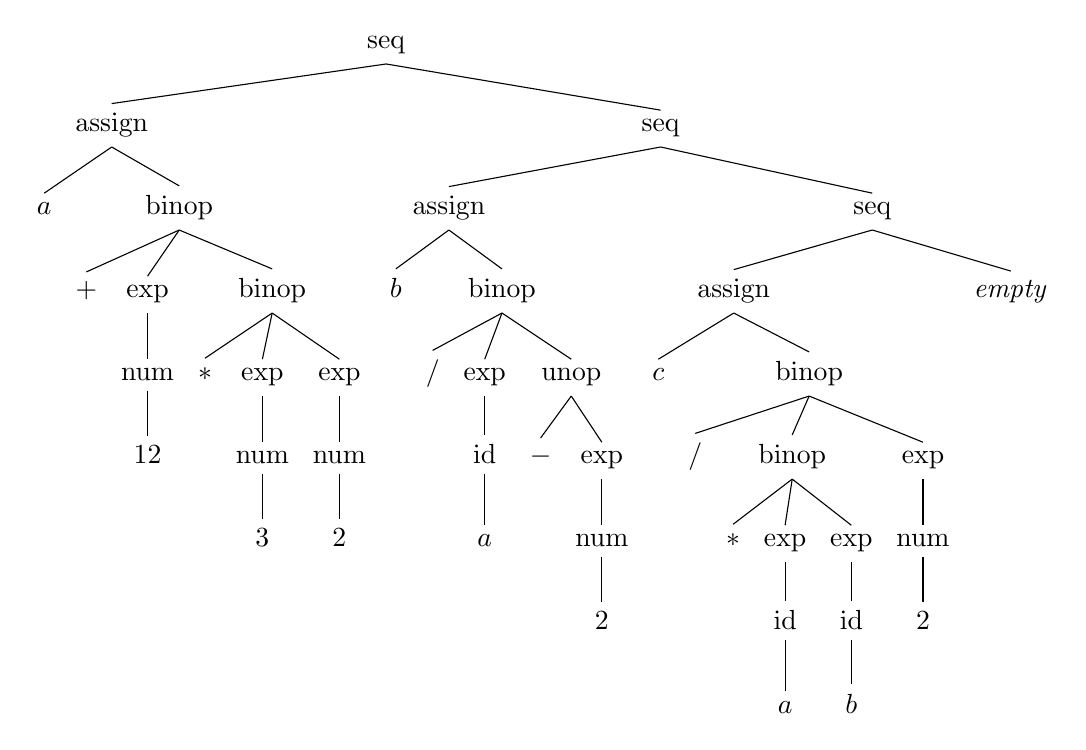
\begin{tikzpicture}
\Tree [.seq 
[.assign $a$ [.binop $+$ [.exp [.num $12$ ] ]
[.binop $*$ [.exp [.num $3$ ] ]
[.exp [.num $2$ ] ]
 ]
 ]
 ]
[.seq 
[.assign $b$ [.binop $/$ [.exp [.id $a$ ] ]
[.unop $-$ [.exp [.num $2$ ] ]
 ]
 ]
 ]
[.seq 
[.assign $c$ [.binop $/$ [.binop $*$ [.exp [.id $a$ ] ]
[.exp [.id $b$ ] ]
 ]
[.exp [.num $2$ ] ]
 ]
 ]
[.\emph{empty} ]
] 
] 
] 
\end{tikzpicture}
\end{document}
